Avant de discrétiser les Laplaciens de nos deux images, il faut définir le maillage que nous allons utiliser.
 
\subsubsection{Qu'est qu'une image}
Une image peut être représentée comme une succession de pixels. En traitement d'image, ce sont d'ailleurs sur ces pixels que le traitement est effectué. Leur modification entraîne la modification de l'image globale.Nous verrons donc une image comme la succession de pixels et nous pouvons la représenter comme une grille, dans laquelle chaque carré représente un pixel.  Schématiquement, nous pourrions donc découper notre image comme ci-dessous
    \begin{figure}[!htb]
        \centering
       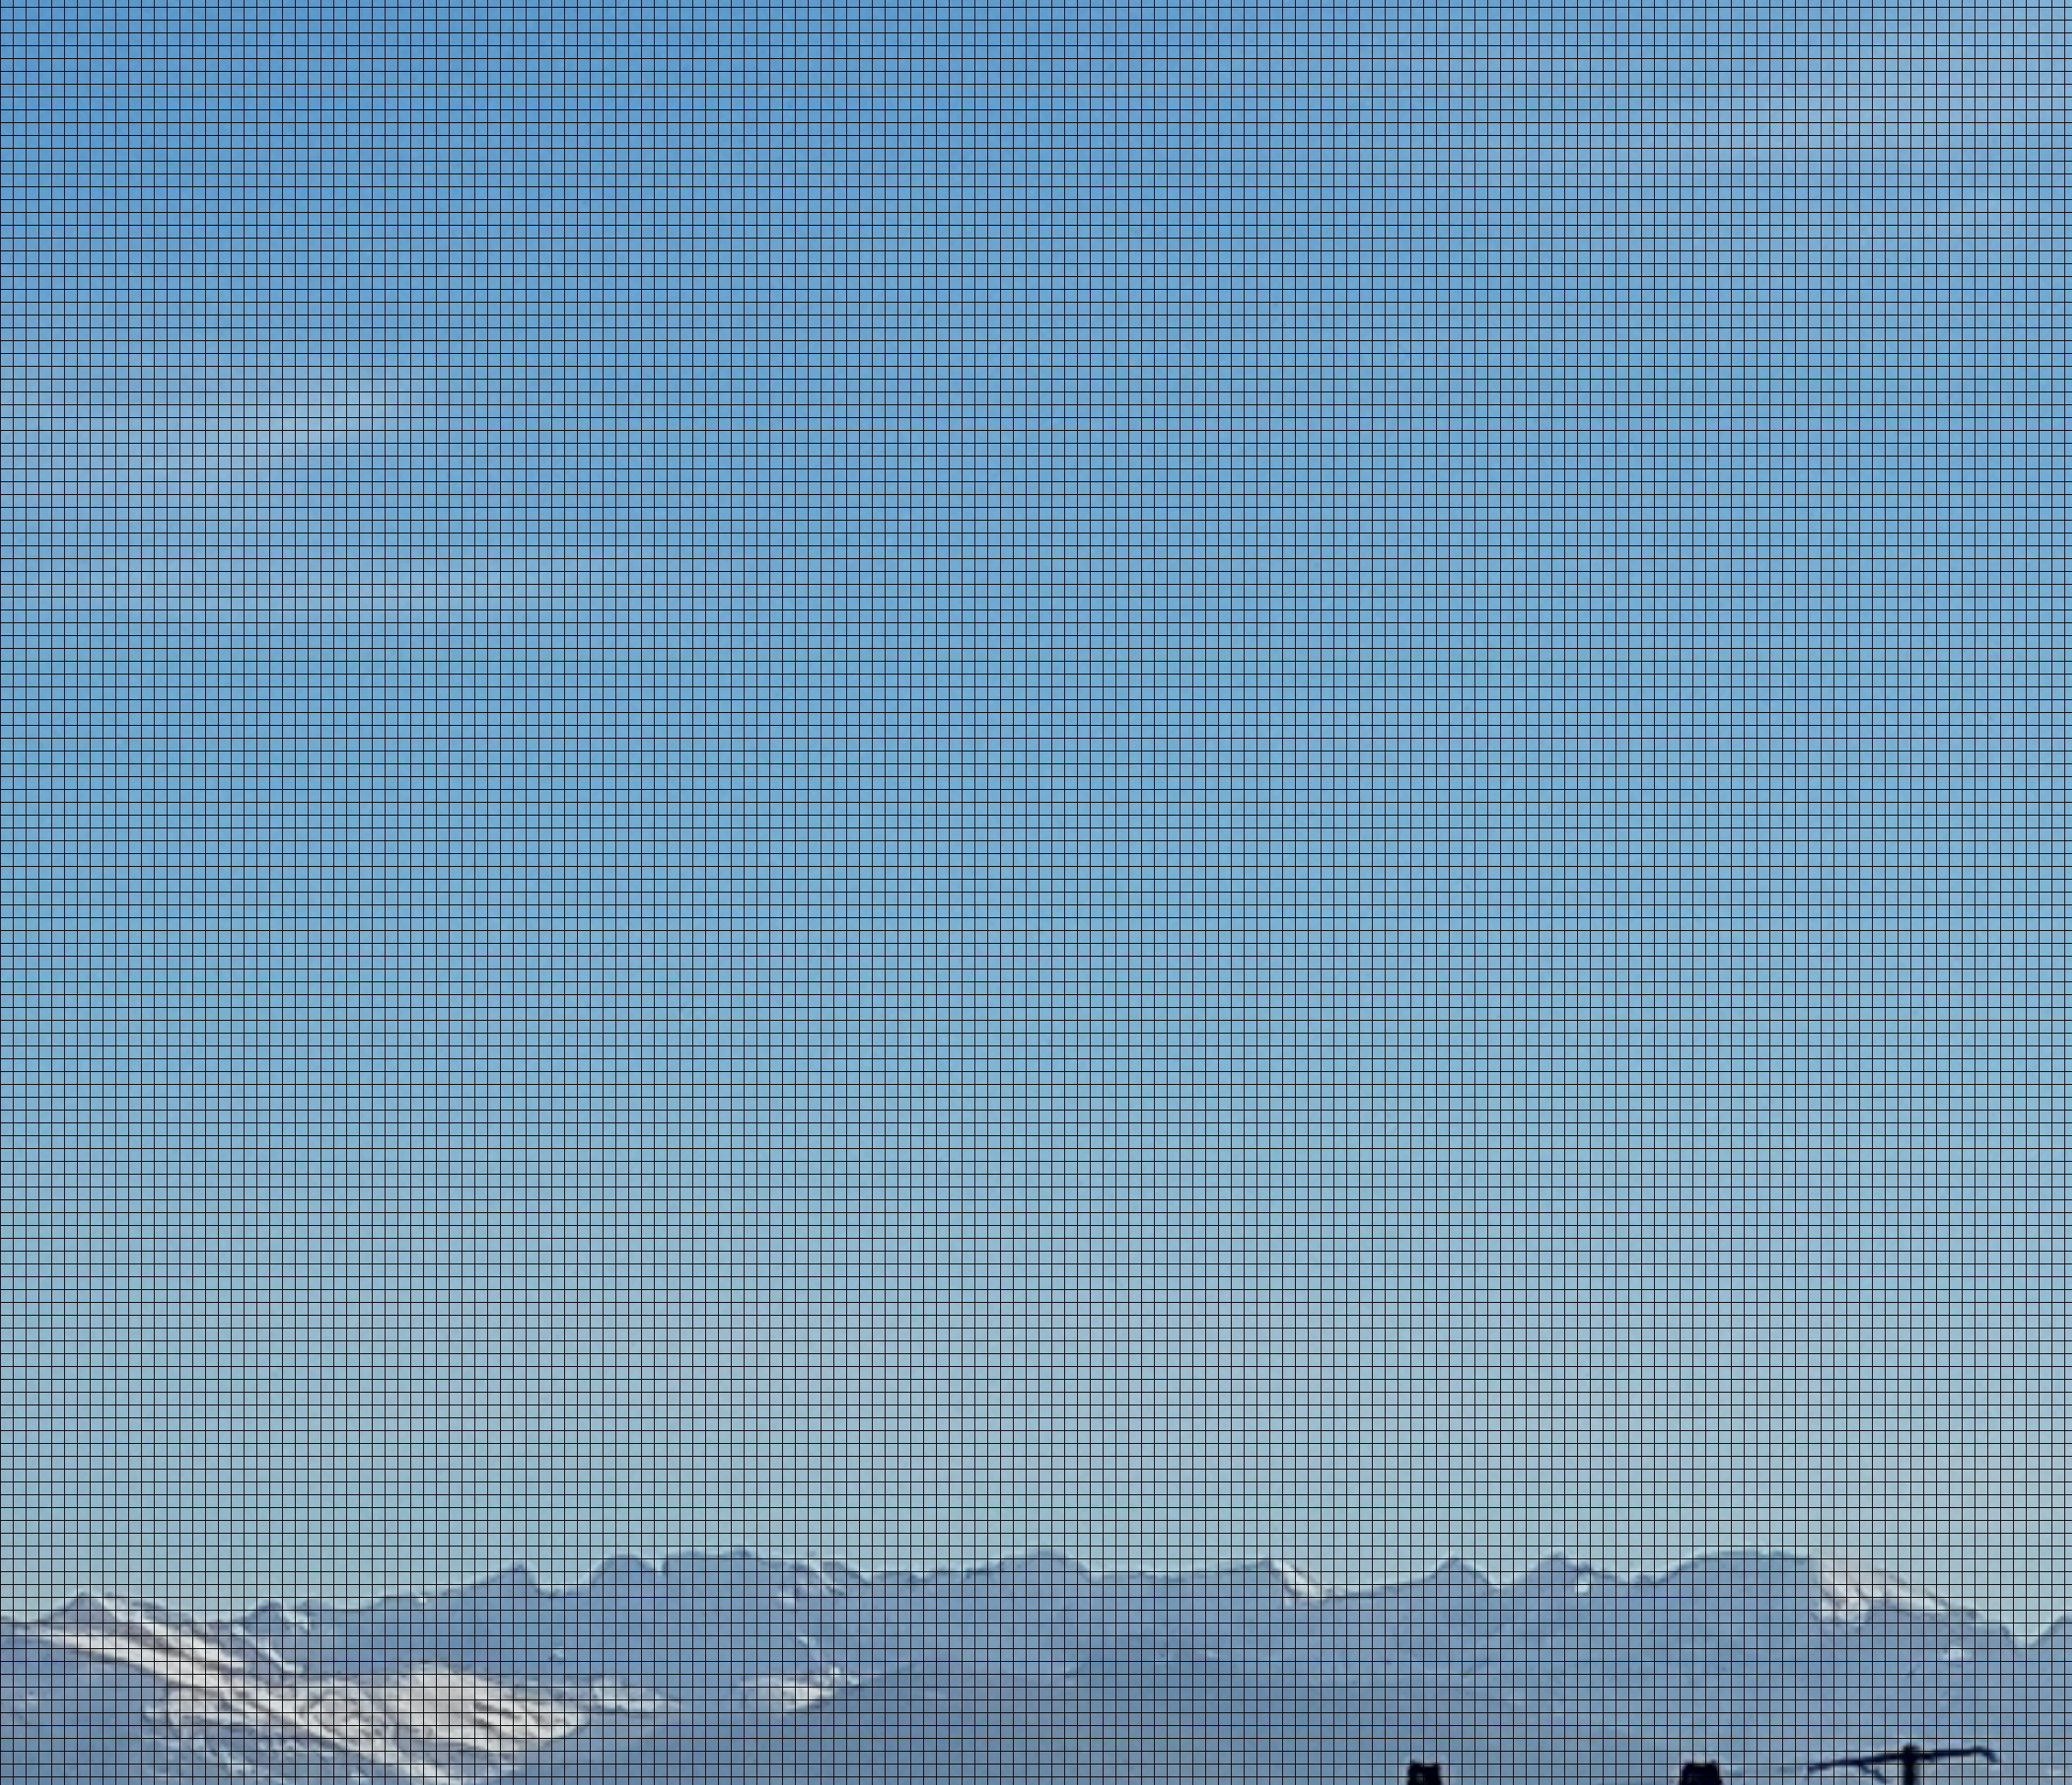
\includegraphics[scale = 0.07]{Images/Montagne_grille.jpg}
        \caption{Maillage d'une image}
        \label{fig:my_label}
    \end{figure}
Nous numéroterons les pixels suivant la règle suivante. Le premier pixel est situé en haut en gauche, puis il suffit de parcourir la grille comme ci-dessous : 

	\begin{figure}[!htb]
	\centering
	
\includegraphics[scale=0.5]{Images/grille.jpg}
	\caption{Parcours d'une grille}
	\label{fig:my_label}
	\end{figure}
Les pas d'espaces sont donc égaux et valent 1. Dans la suite nous considérons que notre image est de taille $N \times M$.
\newpage


\subsection{Les différents opérateurs nécessaires}
Nous utiliserons certains opérateurs que nous définissons ici afin de ne pas alourdir les différentes sections. 
\subparagraph{Le gradient}

\subparagraph{Le Laplacien}
Le Laplacien peut s'écrire de la forme : 

\begin{center}
\begin{equation*}
    \Delta I(x,y)  = \frac{\partial^2 I}{\partial x^2}+ \frac{\partial ^2 I}{\partial y^2}
\end{equation*}
\end{center}

\subsection{Méthode des différences finies}
Nous cherchons à résoudre  : 
\begin{center}

\begin{equation*}
    \left \{
    \begin{aligned}
    \Delta I = \Delta S \ sur \ \Omega\\
    I = T \ sur \ \partial \Omega
    \end{aligned}
    \right.
\end{equation*}
\end{center}

En utilisant la méthode des différences finie, commençons par discrétiser le Laplacien.
Pour discrétiser celui-ci, il faut donc commencer par discrétiser $\frac{\partial^2 I}{\partial x^2}$ et  $\frac{\partial^2 I}{\partial y^2}$. 

\subparagraph{Discrétisation des dérivées secondes :}

A l'aide des formules de Taylor à l'ordre 2 ci-dessous : 
\begin{equation*}
\begin{aligned}
    I(x+h,y) = I(x,y)+h\times \frac{\partial I(x,y)}{\partial x}+ h^2 \times \frac{\partial ^2 I(x,y)}{\partial x^2} + o(h^3) \\
    I(x-h,y) =I(x,y)- h\times  \frac{\partial I(x,y)}{\partial x}+ h^2 \times \frac{\partial^2 I(x,y)}{\partial x^2} + o(h^3)
\end{aligned}
\end{equation*}


Et en effectuant la somme de ces deux équations, nous obtenons une discrétisation possible de $\frac{\partial ^2 I(x,y)}{\partial x^2}$:  
\begin{equation*}
    \frac{\partial ^2 I(x,y)}{\partial x^2} =\frac{1}{h^2} \times I(x+h,y) + I(x-h,y) - 2\times I(x,y)
\end{equation*}

\subsubsection{Discrétisation du Laplacien}
Comme le Laplacien n'est autre que la somme de $\frac{\partial ^2 I(x,y)}{\partial x^2}$ et$\frac{\partial ^2 I(x,y)}{\partial y^2}$, une discrétisation possible de celui-ci s'écrit de la forme  : 
\begin{equation*}
    \Delta I(x,y) =  \frac{I(x+h,y) + I(x-h,y) - 2\times I(x,y)}{h^2}  + \frac{I(x,y+k) + I(x,y-k) - 2\times I(x,y)}{k^2} \\
\end{equation*}

Les pas d'espaces h et k étant égaux à 1, nous pouvons écrire une discrétisation du Laplacien  :
\begin{equation*}
     \Delta I(x,y) =  I(x+1,y) + I(x-1,y)+ I(x,y+1) + I(x,y-1) - 4\times I(x,y)  \\
\end{equation*}

\subparagraph{Application à une image }
Afin de calculer le Laplacien du pixel I(i,j),il est donc nécessaire d'avoir la connaissance de ses pixels voisins que nous nommerons par la suite U(p), D(own), L(eft), R(ight) pour les pixels I(i-1,j), I(i+1,j), I(i,j-1), I(i,j+1). 

\begin{center}
    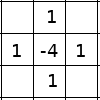
\includegraphics[scale = 0.8]{Images/Laplacian.png}
\end{center}

\subsubsection{Résolution de l'équation de Poisson}
Résoudre $\Delta I(x,y) = \Delta S(x,y)$ sur $\Omega$ est équivalent à résoudre : 
Soit $g(x,y) = S(x+1,y) + S(x-1,y)+ S(x,y+1) + S(x,y-1) - 			4\times S(x,y)$
\begin{center}
\begin{equation*}
    \left \{
    \begin{aligned}
    I(x+1,y) + I(x-1,y)+ I(x,y+1) + I(x,y-1) - 4\times 			I(x,y)= g(x,y)\\ sur \ \Omega \\
    I = T \ sur \ \partial \Omega
    \end{aligned}
    \right.
\end{equation*}
\end{center}

Nous devons donc résoudre un système à $n\times m $ inconnues.

Afin de résoudre ce système, il est plus facile de l'écrire sous forme matricielle. Nous devons donc résoudre un système de la forme AI = b et sa solution est  :  $I = A^{-1}\times b$.
Avec : 
\begin{itemize}
\item A une matrice carrée de taille (mn, mn)
\item I un vecteur colonne de taille (mn,1)
\item b un vecteur colonne de taille (mn,1)
\end{itemize}

\subparagraph{Transformation de l'image}
Afin de pouvoir résoudre ce système, I doit être un vecteur colonne. Or dans notre cas, I est une matrice de taille (m,n). Le nouveau vecteur I, est la concaténation des colonnes de l'image I, comme ci dessous.


\subparagraph{Ecriture de la matrice du système}

\subparagraph{Ecriture de vecteur}
Après avoir calculé le Laplacien de l'image S, le vecteur b est obtenu en concaténant les colonnes de l'image $\Delta S$. 

\subparagraph{Exemple simple}

\begin{center}
    
\includegraphics[width = 200pt]{Images/image_needed.png}
\end{center}
